\label{enhanced methods}


\section{Objective and Theory}
The original metadynamics method presented in Chapter \ref{metadynamics} uses the all atoms spatial coordinates as the reaction coordinates in the metadynamics method.  This results in 3N degrees of freedom, 3 for the spatial coordinates and N for the number of atoms, which leads to super linear increases in computational costs for the metadynamics method.  As shown previously, the cost of applying a penalty function to the system also increases linearly as the number of penalties increases.  As a result, simulating large systems for sufficient penalties is difficult.  Often other applications of metadynamics choose to use a select few crucial reaction coordinates, such as bond angle in proteins or spatial coordinates of atoms of interest.  However, for a homogeneous predefining the reaction coordinates of interest is extremely difficult.  The goal is to reduce the number of coordinates from 3N used as reaction coordinates for metadynamics in order to more efficiently apply penalties.  This reduce the computational cost of each penalty and will lead to more efficient sampling of the landscape.  

\section{Bond Order Parameter Restrained Metadynamics}
There is no universal method for determining the coordinates of interest, however, methods can be developed based on the goal of the simulation.  For studying nucleation and crystal growth, the goal is to sample the energy landscape while driving the system from a high energy amorphous configuration to a low energy crystalline configuration.  We measure structure in the system with the sixth order bond orientational order parameter, as discussed in section \ref{bop_calculation}.  Thus, if we transform our picture of the energy landscape from spatial coordinates to bond orientational order parameter, the penalties are driving the system from low $\bar{q}_6$ values to high values.  With this understanding, we can justify reducing the variable space based on an atom's $\bar{q}_6$.  In algorithmic terms, the system begins uniformly with low $\bar{q}_6$ values.  Then as penalties are applied, some atoms may rearrange preferentially first, leading to regions of high $\bar{q}_6$ values.  If an atoms $\bar{q}_6$ value exceeds some threshold value, we can consider this atom to have already reached the global minimum of the landscape.  Therefore, we can now safely ignore the spatial coordinates of this atom as potential reaction coordinates, and no longer apply penalties to this atom.  The idea being that if nucleation truly begins from a seed and then grows throughout the system, then we can freeze the nucleation sites and allow the remaining atoms to grow onto the nucleation site.  As the cluster grows, we can freeze more atoms, thus as penalties are applied we can continue reducing the variable space until the global minimum is reached and the variable space becomes zero.  The benefit of this method is that it is finite in time, the simulation ends when all atoms are frozen.  Whereas, traditional metadynamics has no deterministic end point and can therefore continue indefinitely.  

We coined this type of on the fly variable reduction, structurally restrained metadynamics, because the system becomes restrained as a function of structure.  We extended our implementation of traditional metadynamics to include structurally restrained metadynamics as an option.  A function was added into GROMACS to compute the bond orientational order parameter during the simulation.  The user can define after how many penalties the structure of the system should be sampled to detect regions of order and freeze them.  This is an option because computation of the bond order parameter scales with system size, and is not a low cost computation, and in general, multiple penalties are required before any large scale rearrangements are apparent in the system.  Thus, computing the bond orientational order parameter on after each penalty application is excessive.  The extension was built that any integer order of the bond orientational order parameter can be calculated, and the nearest neighbor averaged value can be optionally used as well.

To test this method, we applied it to the same monoatomic Lennard-Jones system used in the previous chapters.  The system was composed of 864 atoms, roughly a 27.0 $nm^3$ simulation box.  The system was equilibrated at 120 K, above the freezing temperature for Lennard-Jones argon.  The metadynamics simulation used a penalty height of 1 kJ/mol, a squared penalty width of .1 $nm^2$, a initial minimization step size of .0001.  The system was restrained based on the nearest neighbor averaged, sixth order bond orientational order parameter, $\bar{q}_6$, the structure was computed every 5 penalties applied, the cutoff parameter for nearest neighbor searching for $\bar{q}_6$ was .47 (the value of the first maximum of the pair distribution function, and the minimum structure to freeze was $\bar{q}_6 = .45$.  The results are shown in Figure \ref{bop_final}. 

\begin{figure}[h]
	\centering
	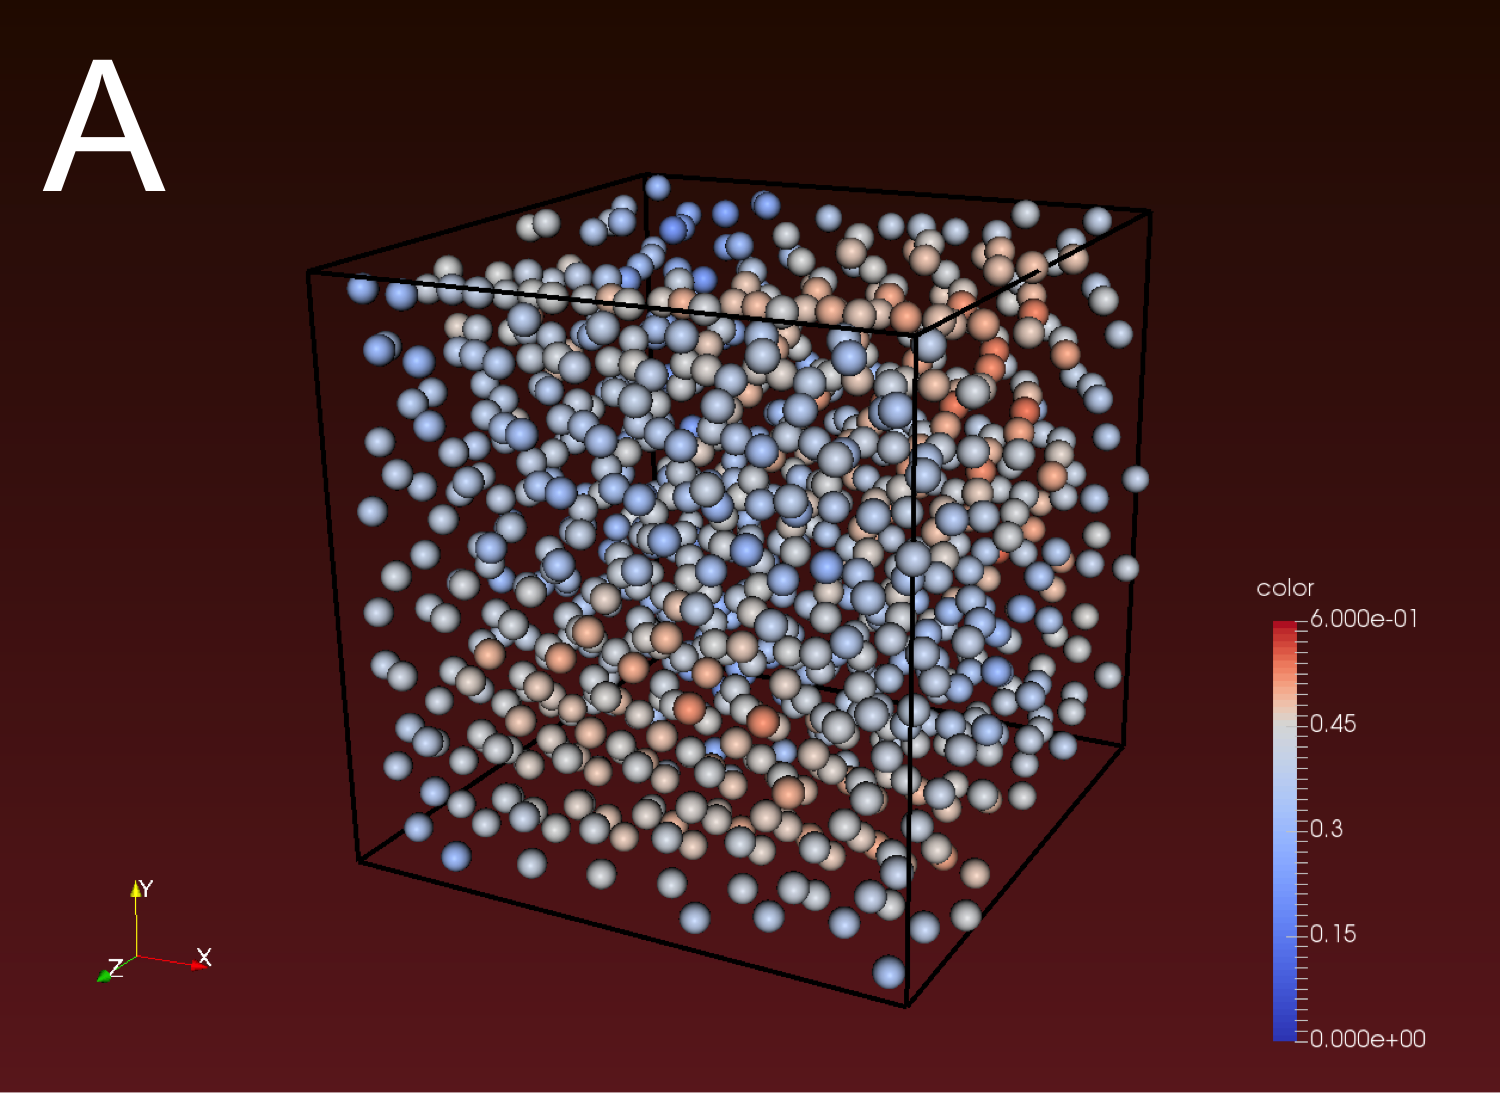
\includegraphics[width = .4\textwidth]{./Figures/Appendix/bop_restrain.png}
	\hspace{.1\textwidth}
	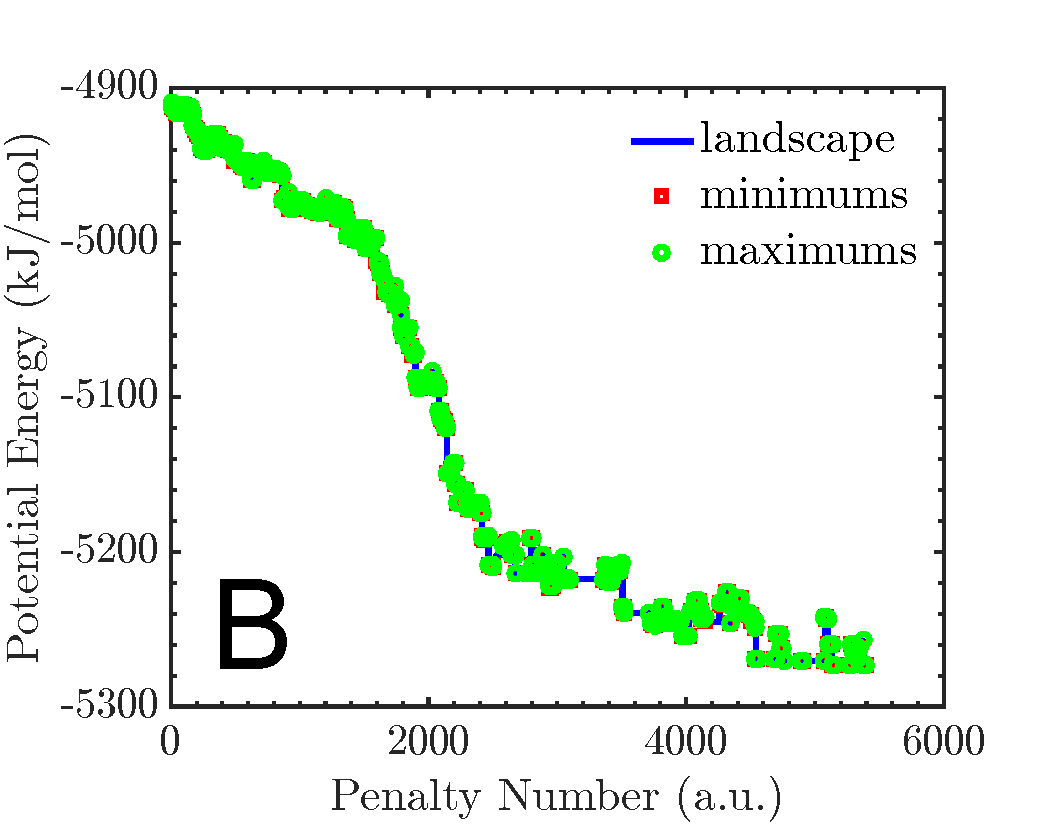
\includegraphics[width = .4\textwidth]{./Figures/Appendix/bop_landscape.pdf}
	\\
	\vspace{5mm}
	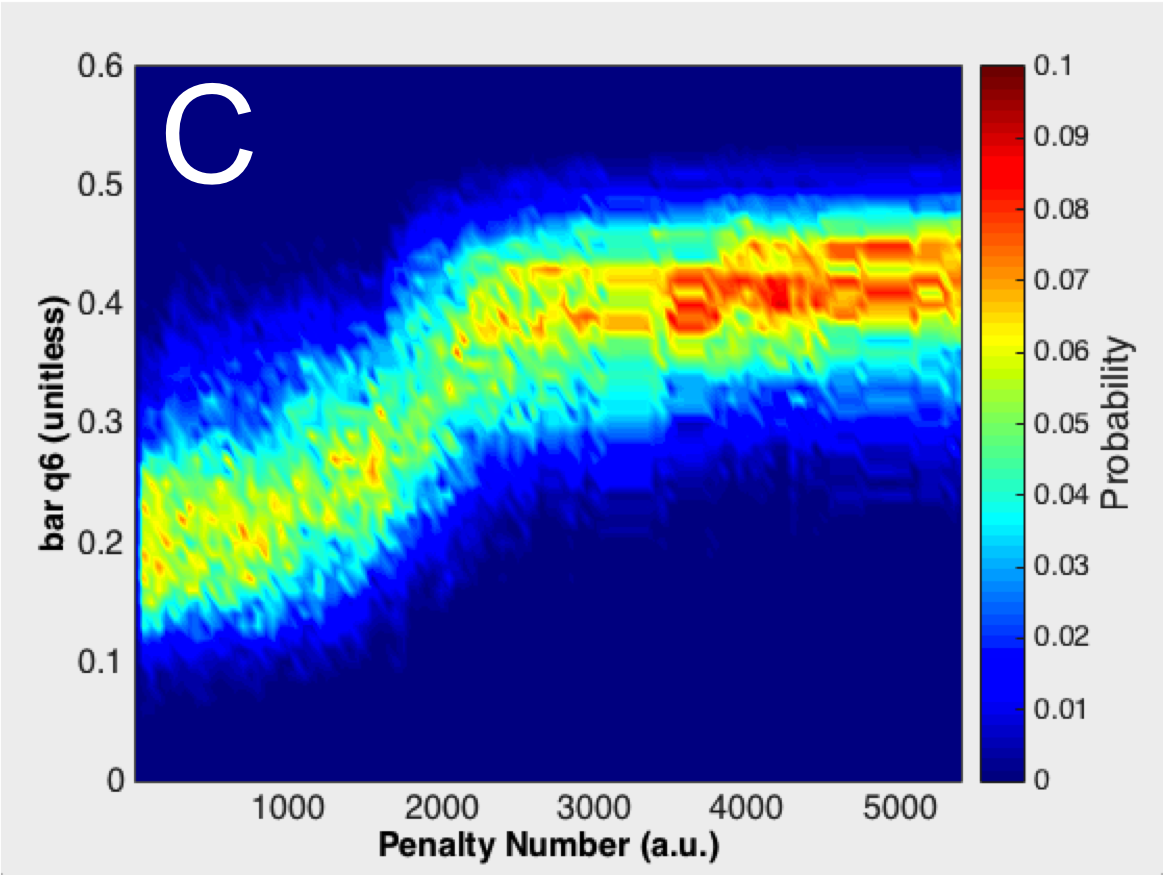
\includegraphics[width = .4\textwidth]{./Figures/Appendix/bop_heatplot.png}
	\caption{Results of a bond order parameter restrained, metadynamics simulation.  Figure A shows the final coordinates of the system after the simulation completed.  The atoms are colored by the $\bar{q}_6$ value, blue representing unordered and red representing ordered.  The figure shows some atoms have achieved moderate ordering but a majority of the atoms are still unordered, and the unordered atoms are clustered together.  Figure B shows the potential energy of the system as a function of penalty during the simulation.  The figure shows a minimum system energy of around -5250 kJ/mol, compared to -5900 kJ/mol for the unrestrained metadynamics method.  Figure C shows the distribution of $\bar{q}_6$ values as a function of penalty applied.  The figure shows that there is a structural transition around 2000 penalties, but the system never attains more than moderate structure values of $\bar{q}_6$.}
	\label{bop_final}
\end{figure}

Figure \ref{bop_final} shows the results of a structurally restrained metadynamics simulation.  Figure \ref{bop_final}A shows the final configuration of the system after the simulation, and compared to traditional metadynamics the order of structure is clearly much lower.  During the simulation, approximately a third of the atoms are restrained by the end of the simulation.  From the movie of the simulation, after around 2000 penalties a group of atoms achieve moderate structure (greater than .45 the threshold value) and are frozen.  However, we know realized that by freezing these atoms and removing degrees of freedom from the simulation, the energy landscape coarsens.  As a result, a majority of the system no longer has the ability to overcome the barriers necessary to achieve order themselves.  So, our hypothesis was correct in that the structurally retained metadynamics resulted in more penalties applied, however, we had not considered that by removing select degrees of freedom we would also remove the ability to form a perfect crystal.  

\section{Bond Order Parameter Restrained, with the Option to Unfreeze, Metadynamics}
While analyzing the structurally restrained metadynamics results, we noticed that many atoms that were frozen would loose structure as more penalties are applied (particularly atoms on the edge of a frozen cluster).  The unfrozen atoms near the surface would continue to rearrange as penalties were applied resulting in frozen atoms on the edge of cluster to have structural values dip back below the threshold value.  Because of this, we created the structurally restrained metadynamics with dynamic unfreezing.  We added the ability for frozen atoms to become unfrozen during the simulation if they lost their structure.  With this method we would dynamically add and remove reaction coordinates as they became relevant.

To test this method, we applied it to the same monoatomic Lennard-Jones system used in the previous chapters.  The system was composed of 864 atoms, roughly a 27.0 $nm^3$ simulation box.  The system was equilibrated at 120 K, above the freezing temperature for Lennard-Jones argon.  The metadynamics simulation used a penalty height of 1 kJ/mol, a squared penalty width of .1 $nm^2$, a initial minimization step size of .0001.  The system was restrained based on the nearest neighbor averaged, sixth order bond orientational order parameter, $\bar{q}_6$, the structure was computed every 5 penalties applied, the cutoff parameter for nearest neighbor searching for $\bar{q}_6$ was .47 (the value of the first maximum of the pair distribution function, and the minimum structure to freeze was $\bar{q}_6 = .45$.  The results are shown in Figure \ref{unfreeze_final}. 

\begin{figure}[h]
	\centering
	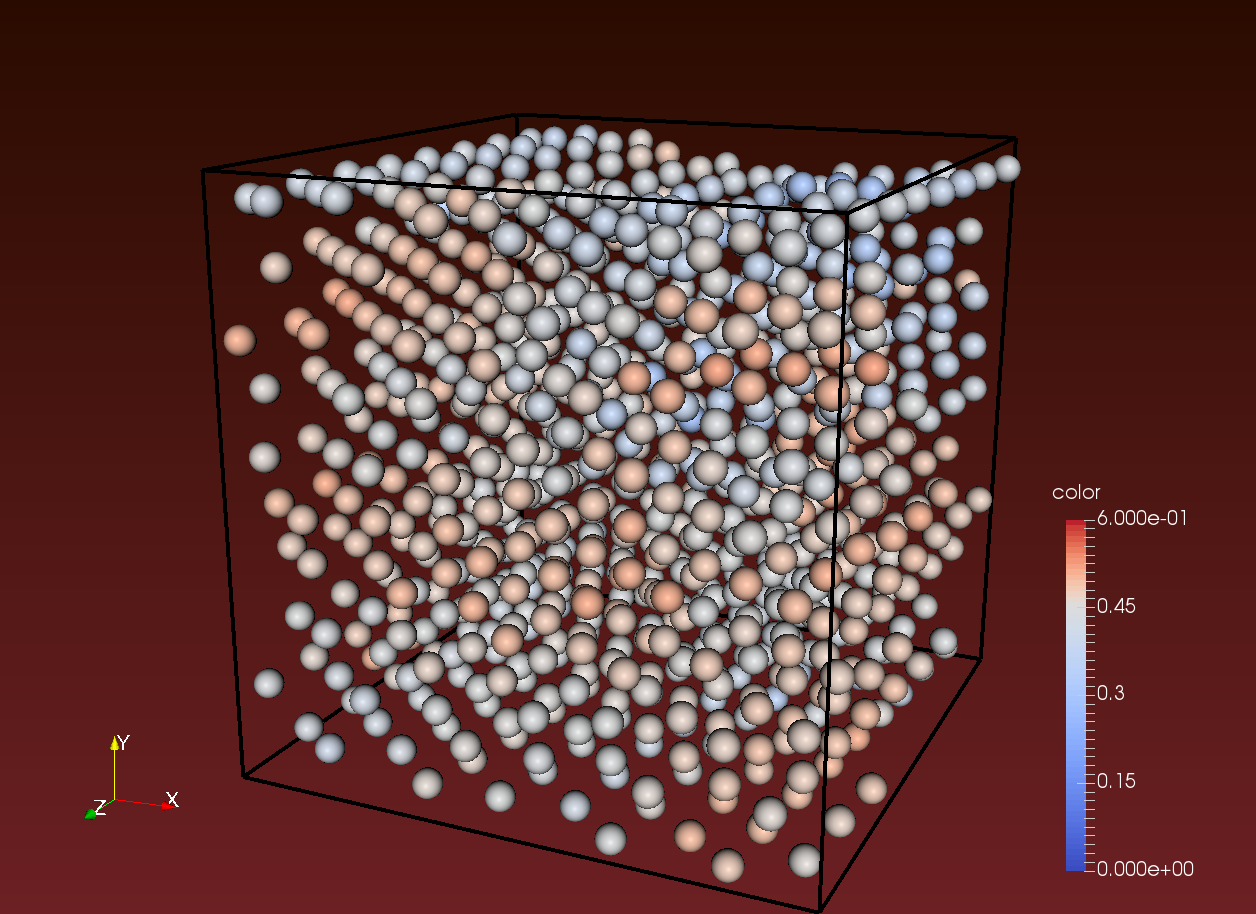
\includegraphics[width = .4\textwidth]{./Figures/Appendix/can_unfreeze.png}
	\hspace{.1\textwidth}
	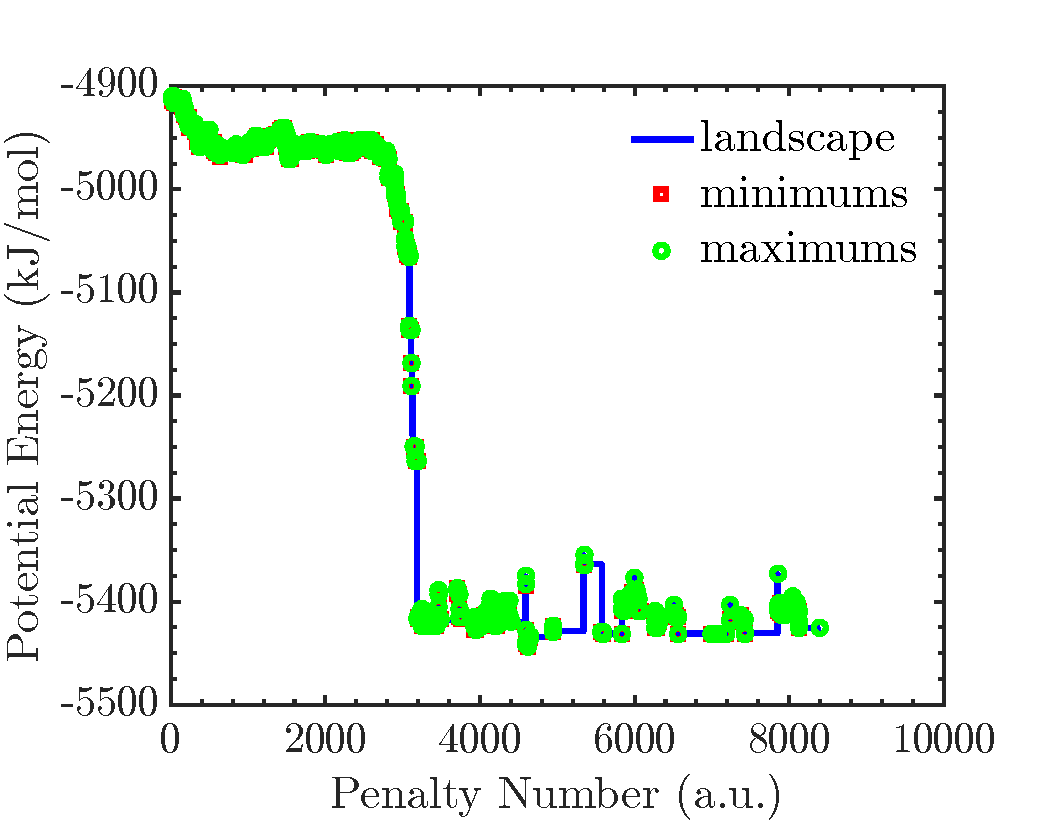
\includegraphics[width = .4\textwidth]{./Figures/Appendix/unfreeze_landscape.pdf}
	\\
	\vspace{5mm}
	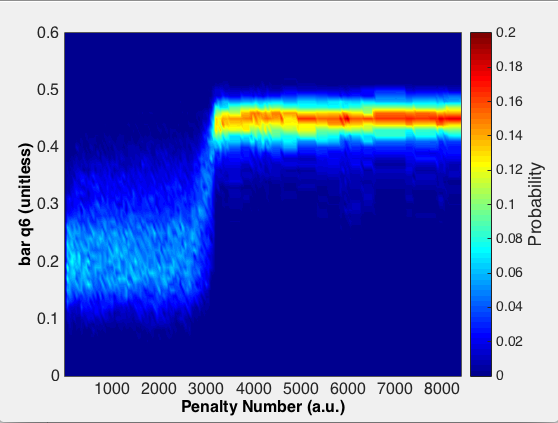
\includegraphics[width = .4\textwidth]{./Figures/Appendix/unfreeze_heatplot.png}
	\caption{Results of a bond order parameter restrained, with the option to unfreeze, metadynamics simulation.  Figure A shows the final coordinates of the system after the simulation completed. The atoms are colored by the $\bar{q}_6$ value, blue representing unordered and red representing ordered.  The figure shows that the majority of atoms have achieved moderate order (roughly .45 $\bar{q}_6$) and that a select few clustered atoms have low order.  Figure B shows the potential energy of the system as a function of penalty during the simulation.  The shows a minimum system energy of around -5450 kJ/mol compared to -5900 kJ/mol for the unrestrained metadynamics method.  Figure shows the distribution of $\bar{q}_6$ values as a function of penalty applied.  The figure shows that there is a structural transition around 3000 penalties, but the system never achieves high $\bar{q}_6$ values. }
	\label{unfreeze_final}
\end{figure}

Figure \ref{unfreeze_final} shows the results of a structurally restrained metadynamics with dynamic unfreezing simulation.  From the figure, it is clear that the dynamic unfreezing allowed for the system to achieve greater structure, the system appears to be in a polycrystalline state.  The simulation resulted in roughly half the atoms freezing.  Like without unfreezing, the method resulted in more penalties applied however, it was not a deterministic simulation like we expected.  Further, the dynamic unfreezing allowed the system to achieve a more consistent structural order, the standard devaition of $\bar{q}_6$ values is far smaller than without unfreezing.  

These two methods because the system was unable to fully crystallize into a single crystal showed us that unlike the typical concept of CNT that atoms merely join or break off of the surface, the crystal also has internal motions that allow for the system to expand.  When we removed the degrees of freedom to allow for atoms internal to the cluster to move, the system was unable to grow with the same ease as in traditional metadynamics.  


\section{Steepest Ascent}
Many metadynamics methods rely on Newton's steepest descent in the algorithm to update the system's configuration towards a local minimum on the potential energy landscape.  This method is known to have quick convergence and is a stable algorithm.  The forces that act on the atoms are calculated by Newton's steepest descent which takes the form
\begin{equation}
\mathbf{r}_{i+1} = \mathbf{r}_{i} - \delta \nabla U(\mathbf{r})
\end{equation}
where $\mathbf{r}$ is the system's configuration, $i$ is the iteration index, $\alpha$ is the size of the minimization step, and $U$ is the potential energy of the system.  The goal of metadynamics is to overcome large potential energy barriers separating basins, which is achieved by various methods.  Thus, a non-trivial idea to move along the potential energy landscape is to use the opposite of Newton's steepest descent method or use ``steepest ascent."  The idea being that if steepest descent can bring the system to a minimum, then steepest ascent can bring the system out of deep minimum to a local maximum.  The equation would be
\begin{equation}
	\mathbf{r}_{i+1} = \mathbf{r}_{i} + \delta \nabla U(\mathbf{r})
\end{equation}
Referring to a hypothetical system in 2-D as shown in \ref{landscape filling}, the simulation would look like a roller coaster, Newton's steepest descent to bring the system down from a maximum to a minimum, and ``steepest ascent'' to bring the system to a new maximum. However, when this idea was implemented into GROMACS \cite{GROMACS} and tested, the resulting trajectory showed the ``steepest ascent'' caused the potential energy of the system to grow exponentially to infinity as a result of two atoms overlapping one another, as shown by Figure \ref{ascent_result}.

\begin{figure}[h]
	\centering
	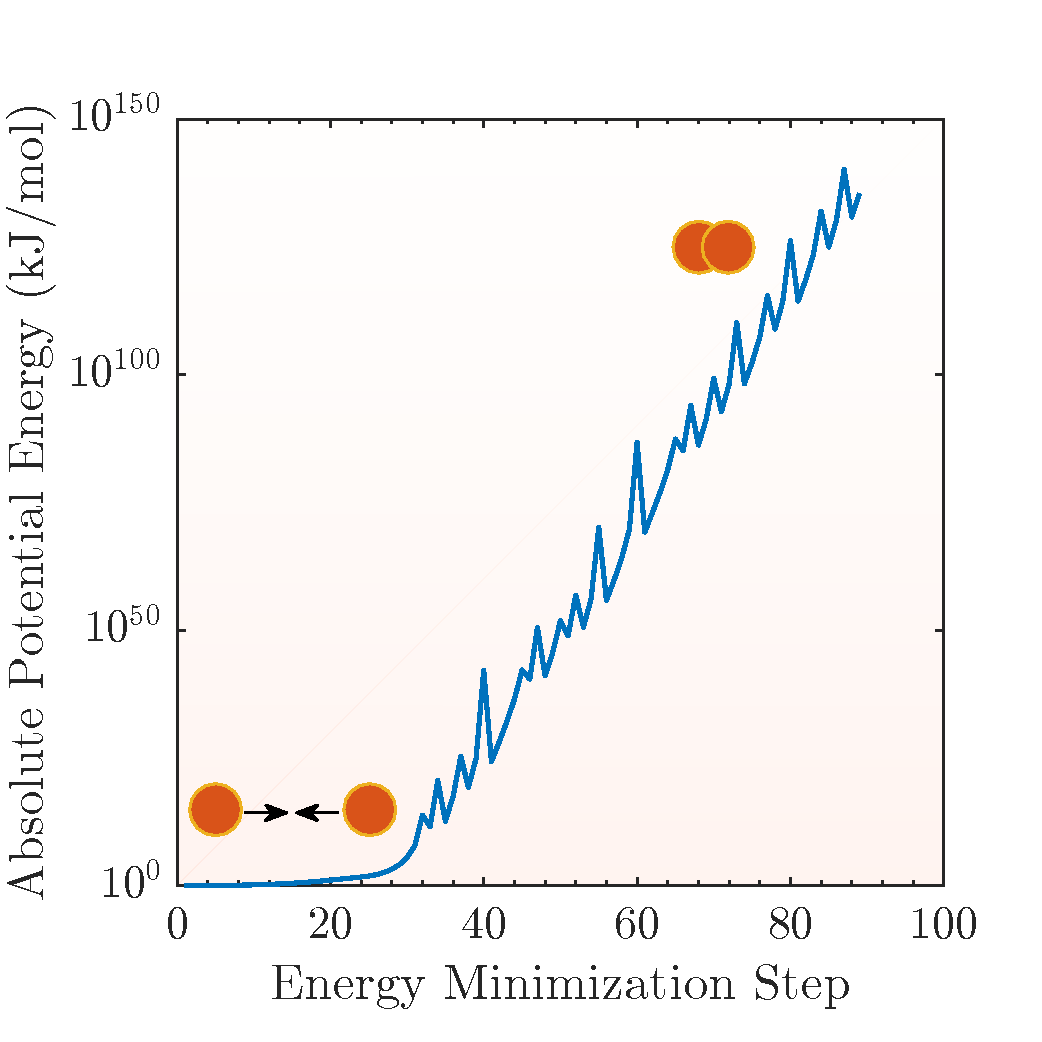
\includegraphics[width=.5\textwidth]{./Figures/Appendix/ascent_result.pdf}
	\caption{Absolute potential energy as a function of energy minimization step for a sample run of steepest ascent implemented in GROMACS.  The simulation is initialized with an NVT equilibrated system of LJ atoms.  The figure shows that at early steps the potential energy begins to rise slowly, as the system crawls from a local minimum.  Here the atoms are well separated and steepest ascent leads to an attractive force.  However, after a local saddle point is crossed, the atoms continue to approach one another at an exponential rate, as shown by the increase in potential energy, eventually leading to overlapping atoms and OFL (infinite) energies.}
	\label{ascent_result}
\end{figure}

Figure \ref{ascent_result} shows the potential energy of the system grows exponentially when plotted in semi-log scale as a function of energy minimization step.  The simulation crashes from OFL or NAN numbers once the atoms start to overlap.  From ``steepest ascent,'' we learned that, while the potential energy landscape is a simple concept when drawn in 2-D (IE vs one reaction coordinate), the energy landscape in 3N-space, as in our simulations, is far more complex than expected.  The landscape is very rich with both small barriers that are rapidly sampled by metadynamics methods but also polluted with infinity large barriers or even walls representing the overlap of two atoms.  Further, the 2-D representation shows metadynamics samples local maxima, which as shown here is an inaccurate picture.  Metadynamics samples minimums and saddle points in the 3N-space landscape.  

We have tried altering and restraining the steepest ascent method to prevent the atoms from overlapping each other.  Various ideas like removing the direction of the largest force, establishing a threshold force that freeze the atoms, etc.  However, steepest ascent is simply a very unstable algorithm because the landscape lacks well defined maximums for the algorithm to converge to.  We still believe this is a viable idea, but further development is required.